\documentclass[12pt,onecolumn,a4paper,fleqn]{article}
\usepackage{epsfig,graphicx,subfigure,amsthm,amsmath}
\usepackage[table,xcdraw,svgnames]{xcolor}
\usepackage{setspace}
\usepackage{mathtools}
\usepackage{fancyhdr}
\usepackage{sidecap}
\usepackage{tikz}
\usepackage{pgfplots}
\usetikzlibrary{decorations.pathreplacing}
\usepackage{relsize}
\usepackage{color,xcolor}
\usepackage[framed,numbered]{matlab-prettifier}
\usepackage{files/persianheader}     
\usepackage{float}
\usepackage{enumerate}
\usepackage{booktabs}
\usepackage{xepersian}


\settextfont[Path=fonts/,BoldFont={ZarBd.ttf},BoldFeatures={Scale=0.9}]{BZar.ttf}

\DeclarePairedDelimiter\ceil{\lceil}{\rceil}
\DeclarePairedDelimiter\floor{\lfloor}{\rfloor}

\definecolor{vgreen}{RGB}{104,180,104}
\definecolor{vblue}{RGB}{49,49,255}
\definecolor{vorange}{RGB}{255,143,102}

\lstdefinestyle{verilog-style}
{
	language=Verilog,
	basicstyle=\small\ttfamily,
	keywordstyle=\color{vblue},
	identifierstyle=\color{black},
	commentstyle=\color{vgreen},
	numbers=left,
	numberstyle=\tiny\color{black},
	numbersep=10pt,
	tabsize=2,
	frame=single,
	literate=*{:}{{\textcolor{black}{:}}}1
}

\lstset{style=verilog-style}



\pagestyle{fancy}
\fancyhf{}
\rhead{\textbf{طراحی سیستم‌های دیجیتال}}
\chead{\textbf{گزارش پروژه}}
\lhead{\textbf{\nouppercase{\rightmark}}}
\cfoot{({\thepage})}
\renewcommand{\headrulewidth}{1pt}
\renewcommand{\footrulewidth}{1pt}
\renewcommand{\sectionmark}[1]{\markright{#1}}
\renewcommand{\subsectionmark}[1]{\markright{#1}}

\onehalfspacing
\begin{document}
%%% title pages
\large
\begin{titlepage}
	
	\begin{center}
		\begin{Large}
			\textbf{
				به نام خدا\\
			}
		\end{Large}
		
		\vspace{2cm}
		
\includegraphics[scale=0.8]{source/sharif1.png}\\
		\vspace{0.5cm}
		\begin{Large}
			\textbf{
				دانشگاه صنعتی شریف\\
				\vspace{0.5cm}
				دانشکده مهندسی کامپیوتر\\
			}
		\end{Large}
		\vspace{2.5cm}
		\begin{huge}
			\textbf{
				طراحی سیستم‌های دیجیتال\\
				\vspace{0.5cm}
			}
		\end{huge}
		
		\begin{Large}
			\textbf{
				پروژه‌ی پایانی درس:\\ ضرب‌کننده‌ی ماتریسی با استاندارد \lr{IEEE 754} \\
			}
		\end{Large}
		
		\noindent\rule[1ex]{\linewidth}{1pt}
		\vspace{1.5cm}
		\begin{Large}{
				استاد:
				\textbf{
					دکتر فرشاد بهاروند \\
				}
				عماد زین‌اوقلی، مازیار شمسی‌پور، بردیا محمدی، جواد هزاره، پویا یوسفی
				
				\vspace{1.5cm}
				\textbf{\today}
			}
		\end{Large}
		
	\end{center}
	\thispagestyle{empty}
\end{titlepage}	

\pagebreak

\tableofcontents
\thispagestyle{empty}
\pagebreak


\section*{شرح وظایف}
\markright{شرح وظایف}


\pagebreak



\section{مقدمه}
	
	\subsection{تعریف الگوریتم}
	الگوریتم مورد استفاده الگوریتم ضرب ماتریسی \lr{Cannon} می‌باشد در این الگوریتم با تقسیم کردن ماتریس‌های ورودی و خروجی به بلاک‌های $k*k$ که در آن $k$ عدد ثابتی می‌باشد می‌خواهیم با داشتن تعدادی پردازنده‌ که به صورت موازی کار می‌کنند عملیات ضرب ماتریسی را بهبود ببخشیم. به طور مثال ماتریس‌ها زیر را در نظر بگیرید:
	\begin{equation}
	A = \begin{bmatrix}
	A_{11}& A_{12}& \dots A_{1\mu}\\
	\vdots& \ddots& \vdots\\
	A_{\lambda1}& A_{\lambda2}& \dots A_{\lambda\mu}\\
	\end{bmatrix} 
	\ \ \, 
	B = \begin{bmatrix}
	B_{11}& B_{12}& \dots B_{1\gamma}\\
	\vdots& \ddots& \vdots\\
	B_{\mu1}& B_{\mu2}& \dots B_{\mu\gamma}\\
	\end{bmatrix} 
	\end{equation}
	
	که در آن هر $A_{ij} و B_{ij}$ یک بلاک $k*k$ می‌باشد.(توجه می‌کنیم که  سایز‌ ماتریس‌ها اگر بخش‌‌پذیر به $k$ نباشد با اضافه‌ کردن صفر آن را بخش پذیر می‌کنیم) با این اوصاف طبق قاعده‌ی ضرب بلوکی می‌دانیم که بلاک $C_{ij}$ در ماتریس جواب از رابطه‌ی زیر محاسبه می‌شود.
	\begin{equation}
	C_{ij} = \sum_{x=0}^\mu A_{ix}B_{xj}
	\label{1}
	\end{equation}
	
	با داشتن تعداد تعداد مشخصی ضرب کننده‌ی ماتریسی $k*k$ می‌توانیم  به طور موازی با استفاده از آنها  و پخش ‌کردن $C_{ij}$ ها بین پردازنده‌های مختلف حاصل نهایی $A\times B$ را محاسبه کنیم. 

در ادامه‌ی این گزارش از علائم ریاضی‌ای استفاده می‌شود که در اینجا به شرح‌ آنها می‌پردازیم.
	
\pagebreak

\subsection{قرارداد‌های ریاضی}

ورودی الگوریتم مورد استفاده  ماتریس‌های مستطیلی $A_{mr}$ و $B_{rn}$ خواهند بود و بنابراین ماتریس‌ خروجی به صورت
$A_{mr} \times B_{rn} = C_{mn}$
خواهد بود. با این‌ حال در هر کجای گزارش که از عبارت $A_{ij}$ (و همینطور برای $B,C$) استفاده شد منظور بلاک‌ $k*k$ ستون $i$ام و سطر $j$ام می‌باشد. برای روشن‌تر شدن این موضوع به مثال زیر توجه می‌کنیم، فرض کنید ماتریس $A$ به صورت زیر باشد:

	$$ A_{mr} = \begin{bmatrix}
	a_{00}& a_{01}& \dots& a_{0r}\\
	\vdots& \vdots& \ddots& \vdots\\
	a_{m0}& a_{m1}& \dots& a_{mr}
	\end{bmatrix} $$
	
	حال اگر این ماتریس را به بلوک‌های $k*k$ تقسیم کنیم و در صورت لزوم درایه‌های نهایی را صفر قرار دهیم ماتریسی به فرم زیر خواهیم داشت:
	
	$$ A^* = \begin{bmatrix}
	\begin{array}{cccc|c}
		A_{00} & A_{01} & \dots & A_{0\mu-1} &  \\
		\vdots & \vdots & \ddots & \vdots & 0 \\
		A_{\lambda-10} & A_{\lambda-11} & \dots & A_{\lambda\mu-1} & \\
		\hline
			& 0 & & & 0
	\end{array}
	\end{bmatrix} $$
که لازم است که توجه داشته باشیم که وقتی ماتریس‌ها را به فرم بلوکی می‌نویسیم مقادیر زیر را تعریف می‌کنیم:
\begin{subequations}
	\begin{equation}
		\mu = \ceil*{\dfrac{r}{k}}
	\end{equation}    
	\begin{equation}
		\lambda = \ceil*{\dfrac{m}{k}}
	\end{equation}
	\begin{equation}
		\gamma = \ceil*{\dfrac{n}{k}}
	\end{equation}
	\begin{equation}
	\theta = \ceil{\dfrac{\lambda\gamma}{\text{\lr{\#Matrix Processors}}}}
	\end{equation}
	
	\label{2}
\end{subequations}
از این نماد‌ها به کرّات در طول گزارش استفاده خواهد شد. توجه می‌کنیم که علت اینکه سقف این حاصل تقسیم‌ها را در نظر گرفتیم همان است که اگر اندازه‌ی ماتریس‌ها بر $k$ بخش‌پذیر نباشند با اضافه کردن صفر به انتها‌ی آن باعث بخش‌پذیری می‌شویم. 
\subsection{نحوه‌ی عملکرد از نظر مساحت و تایمینگ}
از آنجایی که هر ضرب کننده‌ی ماتریسی در حدود
 $k^3$
 کلاک سایکل زمان می‌برد و محاسبه‌ی هر بلوک $C_{ij}$ با توجه به
 \autoref{1}
به $\mu$ بار به ضرب ماتریسی نیاز دارد. همچنین برای محاسبه‌ی تمام بلوک‌ها باید $\lambda\gamma$ بار محاسبات بالا را انجام دهیم با این حال اگر فرض کنیم که تعداد پردازنده‌ها $p$ باشد آنگاه می‌توانیم ببینیم که تعداد کلاک‌ سایکل‌ها تقریبا برابر با عبارت زیر است:
\begin{equation}
	\dfrac{\lambda\gamma\mu k^2}{\text{\lr{\#number of PU}}} = 	\dfrac{\lambda\gamma\mu k^2}{p}
\end{equation}

همچنین تعداد رجیستر‌هایی که هر واحد ضرب‌کننده‌ی ماتریس مربعی نیاز دارد از $O(k^2)$ می‌باشد. و بنابراین تعداد تمام رجیستر‌هایی که مورد نیاز است از $O(pk^2)$ می‌باشد.

\subsection{استاندارد‌ \lr{IEEE 754}}
محاسبات در این پروژه از استاندارد
 \lr{IEEE 754 - Single-precision floating-point}
 پیروی می‌کند که به طور مختصر به شرح آن می‌پردازیم. \\
 در این استاندارد اعداد اعشار با سه بخش \lr{exponent} , \lr{fraction} , \lr{sign} مشخص می‌شوند که سهم هر یک از آنها مانند مثال زیر است:
 
\begin{figure}[h]
	\centering
	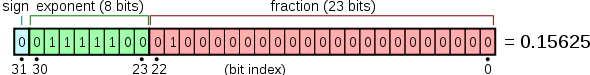
\includegraphics[width=0.8\linewidth]{source/float_example.png}
\end{figure}

و هر عدد طبق فرمول زیر به این نمایش در می‌آید:

\begin{equation}
\text{value} = (-1)^{sign} \times 2^{(E-127)} \times (1 + \sum_{i=1}^{23}b_{23-i}2^{-i})
\end{equation}
\pagebreak
\subsection{کاربرد‌ها}
 
 محاسبات ماتریسی، در سیستمهای پردازش تصویر، در سیستمهای مخابراتی MIMO ،در سیستم های مخابراتی که از روش OFDM برای ارسال اطالاعات استفاده می کنند و همچنین در سیستم های رادار و سونار که مراحل آشکارسازی و تخمین را به کمک اطاعاتی که از آرایه ای از سنسورها جمع آوری شده انجام می دهند، کاربرد فراوانی دارند. 
 واحد ضرب ماتریس در برنامه های پردازش سیگنال دیجیتال مانند تصویربرداری دیجیتال، پردازش سیگنال، گرافیک رایانه ای و چندرسانه ای استفاده می شود. بنابراین بسیار مهم است که مساحت کمتری اشغال کند، سریع کار کند و انرژی کمی مصرف کند. 
 در این پروژه، به چگونگی محاسبه ی ضرب ماتریس ها و پیاده سازی آن، به عنوان یک بخش از مباحث محاسبات ماتریسی پرداخته شده است.

\subsection{مراجع مورد استفاده}

\begin{latin}
\begin{thebibliography}{}
	
	\bibitem{parallel} 
	Abhishek Kumar : Scalability of Parallel Algorithms for Matrix Multiplication
	
	\bibitem{parallel} 
	Patricia Ortega : Parallel Algorithm for Dense Matrix Multipication
	
	\bibitem{area} 
	Ju-wook Jang, Seonil Choi and Viktor K. Prasanna : Area and Time Efficient Implementations of Matrix Multiplication on FPGAs
	
	\bibitem{cannon}
	Cannon's algorithm, Wiki-pedia\\ https://en.wikipedia.org/wiki/Cannon\%27s\_algorithm
	
	
\end{thebibliography}
\end{latin}

\pagebreak

\section{توصیف معماری سیستم}
\subsection{اینترفیس‌های سیستم و قرارداد استفاده از آن }
به طور کلی  و از نگاه بالا سخت‌افزار از یک حافظه و و کمک-پردازنده‌ی ضرب ماتریسی\footnote{\lr{Matrix Multiplier - Co-processor}} تشکیل شده است که پردازنده برای استفاده از‌ می‌تواند ورودی‌ها را درون حافظه قرار داده و خروجی‌ها را نیز از آن بخواند(\lr{I/O Mapped}). 
\\ برای استفاده از این  کمک-پردازنده قرارداد‌هایی در نحوه‌ی استفاده از مموری وجود دارد که باید به آن توجه شود.

\subsubsection{ساختار کلی حافظه} ساختار کلی حافظه به صورت زیر خواهد بود:
\vspace{1cm}
\begin{table}[h]
	\centering
	\begin{tabular}{clll}
		\hline
		\multicolumn{4}{|c|}{Config}                                          \\ \hline
		\multicolumn{4}{|c|}{Status}                                          \\ \hline
		\multicolumn{4}{|c|}{$A_{11}$}                                        \\ \hline

		\multicolumn{4}{|c|}{$A_{12}$}                                        \\ \hline

		\multicolumn{4}{|c|}{$\vdots$}                                        \\ \hline
		\multicolumn{4}{|c|}{$A_{\lambda\mu}$}  \\ \hline   
		\multicolumn{4}{|c|}{$B_{11}$}                                        \\ \hline
		\multicolumn{4}{|c|}{$B_{12}$}                                        \\ \hline
				\multicolumn{4}{|c|}{$\vdots$}                                        \\ \hline
		\multicolumn{4}{|c|}{$B_{\mu\gamma}$}                                        \\ \hline
				\multicolumn{4}{|l|}{\cellcolor[HTML]{595959}{\color[HTML]{595959}aaaaaaaaaaaaaaaaaaaaa }} \\ \hline   
			\multicolumn{4}{|c|}{$C_{11}$}                                        \\ \hline
	
	\multicolumn{4}{|c|}{$C_{12}$}                                        \\ \hline
	
	\multicolumn{4}{|c|}{$\vdots$}                                        \\ \hline
	\multicolumn{4}{|c|}{$C_{\lambda\gamma}$}  \\ \hline 
	    				\multicolumn{4}{|l|}{\cellcolor[HTML]{595959}{\color[HTML]{595959}aaaaaaaaaaaaaaaaaaaaa }} \\ \hline   
	\end{tabular}
	\caption{شماتیک حافظه}
\end{table}
\vspace{1cm}

که در آن هر یک از $A_{ij} , B_{ij} , C_{ij}$ها یک بلوک $k*k$ خواهند بود و باید آن‌ها را به صورت سطری در خانه‌های پشت سر هم حافظه نوشت. 

\pagebreak
برای مثال اگر ماتریس‌های 
$B,A$ به صورت زیر باشند:
$$ A = \begin{bmatrix}
1& 2 & 3\\
4& 5 & 6
\end{bmatrix} , 
B = \begin{bmatrix}
1& 2 \\
3& 4 \\
5& 6
\end{bmatrix}
$$
و ماتریس خروجی به صورت 
$ C = \begin{bmatrix}
22& 28 \\
48& 64
\end{bmatrix}
 $
 خواهد بود. در صورتی که 
$k=2$
و به عبارتی واحد‌های درونی ضرب کننده‌های ماتریس مربعی ما توانایی ضرب بلوک‌های $2*2$ را داشته‌ باشند؛ \lr{CPU} باید آن را به صورت زیر در حافظه قرار دهد و همچنین بلوک‌های خروجی را از بخش‌های مشخص شده استخراج کند:
:
\begin{table}[h]
	\centering
	\begin{tabular}{clll}
		\hline
		\multicolumn{4}{|c|}{Config}                                          \\ \hline
		\multicolumn{4}{|c|}{Status}                                          \\ \hline
		\multicolumn{4}{|c|}{1}                                        \\ \hline
		\multicolumn{4}{|c|}{2}                                        \\ \hline
		\multicolumn{4}{|c|}{4}                                        \\ \hline
		\multicolumn{4}{|c|}{5}                                        \\ \hline
		
		\multicolumn{4}{|c|}{3}                                        \\ \hline
				\multicolumn{4}{|c|}{0}                                        \\ \hline
					\multicolumn{4}{|c|}{6}                                        \\ \hline
										\multicolumn{4}{|c|}{0}                                        \\ \hline
		\multicolumn{4}{|c|}{1}                                        \\ \hline
		\multicolumn{4}{|c|}{2}                                        \\ \hline
		\multicolumn{4}{|c|}{3}                                        \\ \hline
		\multicolumn{4}{|c|}{4}                                        \\ \hline
		\multicolumn{4}{|c|}{5}                                        \\ \hline
		\multicolumn{4}{|c|}{6}                                        \\ \hline
		\multicolumn{4}{|c|}{0}                                        \\ \hline
		\multicolumn{4}{|c|}{0}                                        \\ \hline
		\multicolumn{4}{|l|}{\cellcolor[HTML]{595959}{\color[HTML]{595959}aaaaaaaaaaaaaaaaaaaaa }} \\ \hline  
		\multicolumn{4}{|c|}{22}                                        \\ \hline
		\multicolumn{4}{|c|}{28}                                        \\ \hline
		\multicolumn{4}{|c|}{48}                                        \\ \hline
		\multicolumn{4}{|c|}{64}                                        \\ \hline
		 \multicolumn{4}{|l|}{\cellcolor[HTML]{595959}{\color[HTML]{595959}aaaaaaaaaaaaaaaaaaaaa }} \\ \hline  
	\end{tabular}
		
	

 	\caption{شماتیک حافظه برای مثال داده‌ شده}
\end{table}
نکته حائز توجه دیگر نقطه‌ی شروع ماتریس‌های خروجی می‌باشد که تنها‌ کافیست توجه شود که به جز دو خانه‌ی اول حافظه بقیه‌ی خانه‌ها به صورت یکسان بین ماتریس‌های ورودی و ماتریس خروجی تقسیم شده‌است. یعنی اگر اندازه‌ی کل مموری را $N$ در نظر بگیریم 
$\ceil{\frac{N-2}{3}}$
خانه به خروجی اختصاص پیدا می‌کند. 
\pagebreak
\subsubsection{خانه‌ی اول حافظه}
 \lr{CPU} 
 باید اولین خانه‌ی حافظه را که مربوط به کانفیگ می‌باشد به صورت زیر از اعداد پر کند:

\begin{table}[h]
	\centering
	\begin{tabular}{cccc}
		\hline
		\multicolumn{1}{|c|}{$\lambda$} & \multicolumn{1}{c|}{$\gamma$} & \multicolumn{1}{c|}{$\mu$} & \multicolumn{1}{c|}{$\theta$} \\ \hline
		$\overbrace{8 \ bits}$ & $\overbrace{8 \ bits}$             & $\overbrace{8 \ bits}$ & $\overbrace{8 \ bits}$                     
	\end{tabular}
\end{table}

که مقادیر این پارامتر‌ها در 
\autoref{2}
مشخص شده است و همچنین باید توجه شود که مقدار $\theta$ نیز از رابطه‌ی زیر محاسبه می‌شود:

برای مثال فرض کنیم که ماتریس‌های $A_{55}$ , $B_{55}$ در اختیار داشته باشیم. همچنین $4$ پردازنده‌ ضرب ماتریسی $3*3$ در اختیار داشته باشیم، پارامتر‌های مد نظر به صورت زیر محاسبه خواهند شد:

\begin{subequations}
	\begin{equation*}
		\lambda = \ceil{\dfrac{m}{k}} = \ceil{\dfrac{5}{3}} = 2\\
	\end{equation*}

	\begin{equation*}
		\gamma = \ceil{\dfrac{m}{k}} = \ceil{\dfrac{5}{3}} = 2\\
	\end{equation*}

	\begin{equation*}
		\mu =  \ceil{\dfrac{m}{k}} = \ceil{\dfrac{5}{3}} = 2\\
	\end{equation*}

	\begin{equation*}
		\theta = \ceil{\dfrac{\lambda\gamma}{\text{\lr{\#Matrix Processors}}}} = \ceil{\frac44} = 1
	\end{equation*}
	
\end{subequations}

و بنابراین خانه‌ی اول حافظه در هنگامی که کمک-پردازنده دستور شروع به کار را دریافت می‌کند باید به صورت زیر باشد:

\begin{latin}
\begin{table}[h]
	\centering
	\begin{tabular}{cccc}
		\hline
		\multicolumn{1}{|c|}{$0000 0001$} & \multicolumn{1}{c|}{$0000 0010$} & \multicolumn{1}{c|}{$0000 0010$} & \multicolumn{1}{c|}{$0000 0010$} \\ \hline                 
	\end{tabular}
\end{table}
\end{latin}


\subsubsection{خانه‌ی دوم حافظه}


همچنین دومین خانه‌ی حافظه که مربوط به \lr{Status} می‌باشد مطابق شکل زیر می‌باشد.

\begin{latin}
\begin{table}[h]
	\centering
	\begin{tabular}{|c|c|c|c|c|}
		\hline
		\lr{CPU Ready} & \lr{C-P Acknowledge} & $\dots$ &\lr{CPU Acknowledge} & \lr{C-P Ready}\\ \hline
	\end{tabular}
\end{table}
\end{latin}
وظیفه‌ی \lr{CPU} این است که بعد از قرار دادن ورودی‌ها و تنظیم کردن \lr{Config} مقدار بیت \lr{CPU Ready} را فعال کند و بعد از این که بیت \lr{Acknowledge} را از طرف کمک-پردازنده دریافت کرد به کارش ادامه دهد بعد از تمام شدن عملیات  ضرب ماتریسی بیت \lr{C-P Ready} فعال می‌شود و \lr{CPU} می‌تواند بلاک‌های ماتریس خروجی را از مکانی که در مموری مربوط به خروجی‌ها می‌باشد استخراج کند.

\subsubsection{نحوه‌ی دسترسی به حافظه}
برای دسترسی به حافظه تمامی ماژول‌های موجود در سیستم و همچنین \lr{CPU} از یک \lr{Round-Robin Arbiter} استفاده می‌کنند، با این تفسیر که ماژولی بخواهد خط‌های متصل به حافظ\footnote{\lr{Memory Bus}}را تغییر دهد باید از \lr{Arbiter} اجازه‌ی دسترسی بگرد. و اگر \lr{Arbiter} سیگنال \lr{Grant} مربوط به آن ماژول را فعال کرد اجازه‌ی نوشتن روی حافظه در اختیار آن ماژول قرار می‌گیرد. برای روشن‌تر شدن این موضوع خوب است به شماتیک زیر توجه کنید:

\begin{figure}[h]
	\centering
	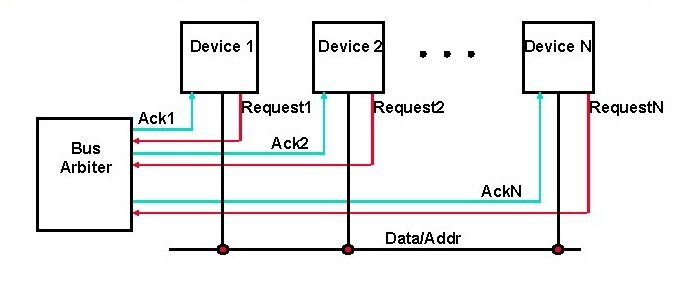
\includegraphics[width=0.5\linewidth]{source/arbiter.jpg}
	\caption{\lr{Arbiter}}
	\label{arbiter}
\end{figure}

\subsubsection{ریست آسنکرون}
سخت‌افزار دارای یک سیگنال \lr{reset} آسنکرون می‌باشد که تمام رجیستر‌های درونش را صفر می‌کند.


\subsubsection{کلاک سخت‌‌افزار}
تمامی ماژول‌های این سخت‌افزار از جمله مموری و تمام ماژول‌های واحد حساب‌کننده‌ی ضرب ماتریسی به صورت سنکرون عمل می‌کنند و \lr{CDC} در این سخت‌افزار اتفاق نمی‌افتد.

\pagebreak

ابتدا ساختار درختی سخت‌افزار طراحی شده را می‌بینیم و سپس به مفسراً درباره‌ی نقش و عملکرد هر یک از ماژول‌های مربوطه صحبت خواهیم کرد.
\subsection{ساختار درختی سیستم}

\begin{figure}[h]
	\centering
	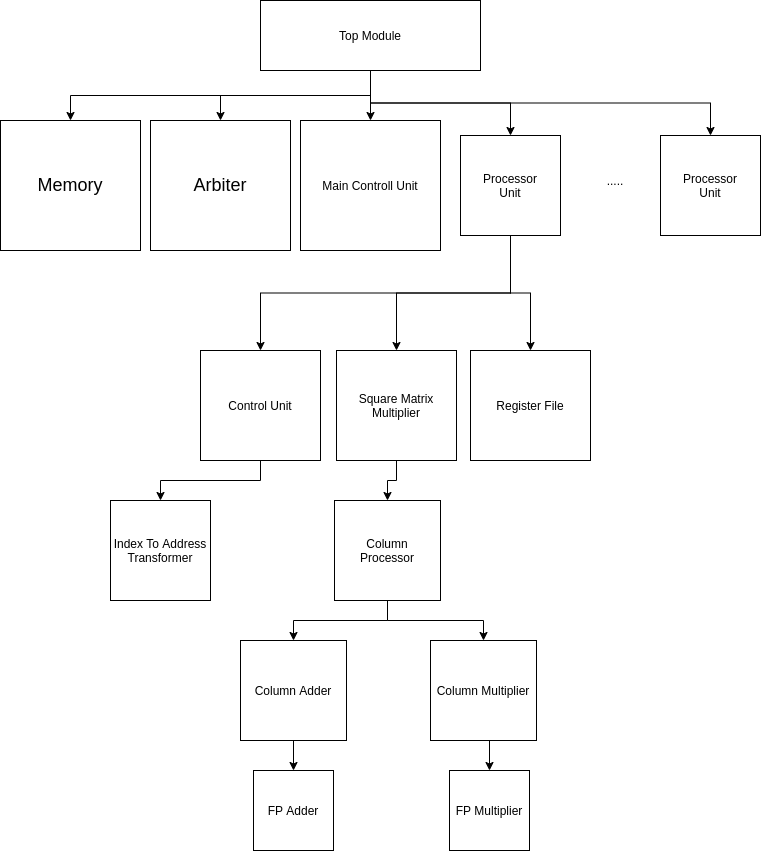
\includegraphics[width=0.87\linewidth]{source/tree.png}
	\caption{\lr{Design Hierarchy}}
\end{figure}

\pagebreak
	
\subsection{توصیف ماژول‌ها}

\begin{itemize}
	\item 
	\lr{Memory}
	
	\begin{figure}[h]
		\centering
		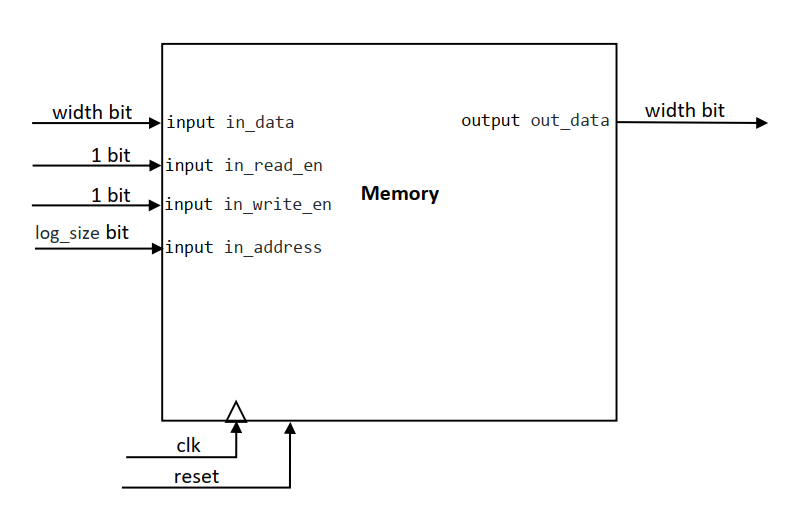
\includegraphics[width=0.6\linewidth]{source/Memory.png}
		\caption{\lr{Memory Schematic}}
	\end{figure}
	
	واحد حافظه سخت‌افزار که مطابق با استانداردی که در بخش‌های قبل مفسراً درباره‌ی آن توضیح دادیم می‌‌باشد.این واحد توانایی آدرس دهی به هر کلمه‌ را دارد(\lr{Word Addressable}). هر کلمه‌ی آن یک عدد ممیز شناور با استاندار \lr{IEEE 754 - Single Precision} می‌باشد.

خواندن و نوشتن در آن این حافظه به منظور بهبود عملکرد زمانی به گونه‌ایست که در هر بار دسترسی به حافظه به تعداد $k$ کلمه در آن نوشته یا از آن خوانده می‌شود.
	
	هر ماژول دیگر در سخت افزار یا بیرون سخت افزار  برای دسترسی به باس ورودی‌های مموری باید از \lr{Arbiter} اجازه گرفته باشد یعنی مطابق \autoref{arbiter} باید سیگنال \lr{Request} خود را فعال کند و سپس منتظر بماند که سیگنال \lr{Grant} دریافت شود و بعد از آن می‌تواند عملیات‌های نوشتن و خواند روی حافظه را انجام دهد.
	
	از آنجایی که \lr{Config} و \lr{Status} مکررا مورد نیاز ماژول‌ها در برنامه قرار می‌گیرد تصمیم گرفتیم که خواندن و نوشتن این دو (البته فقط نوشتن در \lr{Status}) بدون نیاز داشتن به اجازه‌ی \lr{Arbiter} و توسط \lr{Main Controller} که در ادامه‌ آن را توضیح می‌دهیم صورت بگیرد.
	\pagebreak
	\item 
	\lr{Arbiter}
	
	\begin{figure}[h]
		\centering
		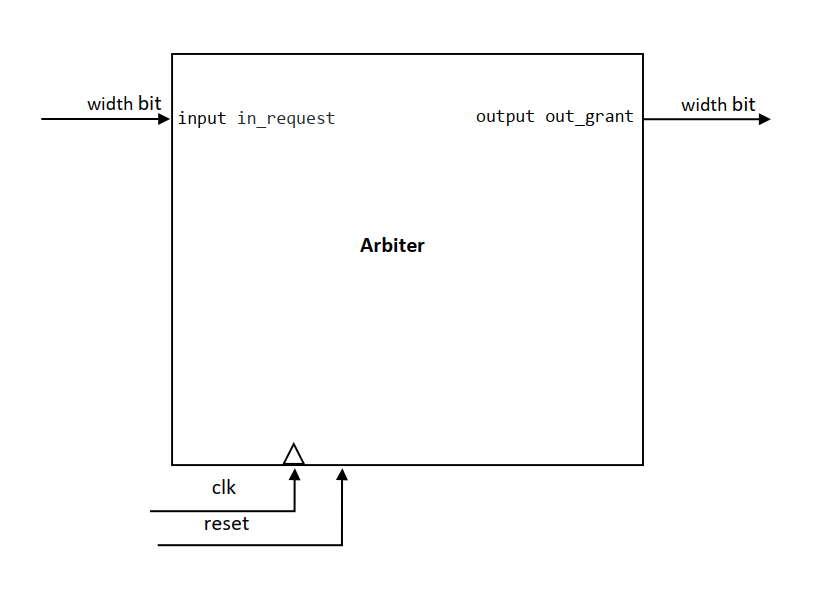
\includegraphics[width=0.4\linewidth]{source/arbiter1.png}
		\caption{\lr{Arbiter Schematic}}
	\end{figure}
	
	همانطور که برای \lr{Memory} توضیح دادیم	این واحد نقش پخش کردن اجازه‌ی دسترسی به مموری را بین ماژول‌ها دارد در \autoref{arbiter}  این موضوع مشخص است. مقدار پهنای ورودی و خروجی این ماژول متناسب با تعداد ماژول‌های دیگریست که اجازه‌ی دسترسی به حافظه را می‌خواهند. برای روشن شدن عملکرد این ماژول به \lr{FSM} زیر توجه کنید:
	
\begin{figure}[h]
	\centering
	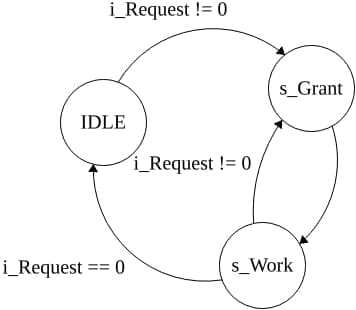
\includegraphics[width=0.4\linewidth]{source/fsm_ar.jpg}
	\caption{\lr{Arbiter Fsm}}
\end{figure}

همانگونه که از این \lr{FSM} مشخص می‌باشد هر گاه یکی سیگنال‌های \lr{Request} فعال  باشد \lr{Arbiter} به حالت \lr{Grant} می‌رود و برای ماژولی که درخواست داده و اولویت بالاتری دارد \lr{Grant} تولید می‌کند. روشن است که سیگنال \lr{Grant}، \lr{Hot-Bit} می‌باشد. وقتی که سیگنال گرنت فعال شد \lr{Arbiter} منتظر می‌ماند که همان ماژولی که \lr{Grant} را دارد \lr{Request} خود را قطع کند. بعد از آن دوباره در صورتی که \lr{Request} داشتن ماژول دیگری به حالت تولید \lr{Grant} می‌رود و در غیر این صورت به حالت اولیه بازگشته و منتظر می‌ماند تا \lr{Request} یکی از ماژول‌ها فعال شود.

\pagebreak

	\item 
\lr{Main Control Unit}

\begin{figure}[h]
	\centering
	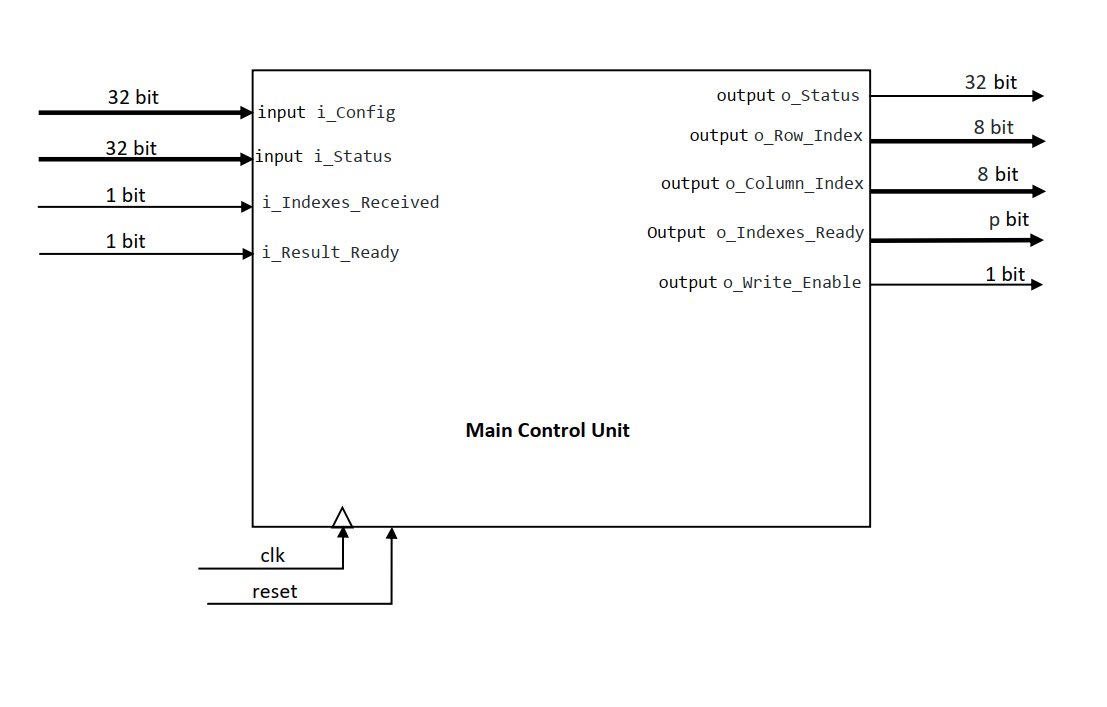
\includegraphics[width=0.6\linewidth]{source/main_cu.png}
	\caption{\lr{Main CU Schematic}}
\end{figure}

این واحد وظیفه‌ی پخش کردن بلاک‌های $C_{ij}$ بین پردازنده‌ها را دارد به نمودار حالت زیر توجه می‌کنیم:
\vspace{0.3cm}

\begin{figure}[h]
	\centering
	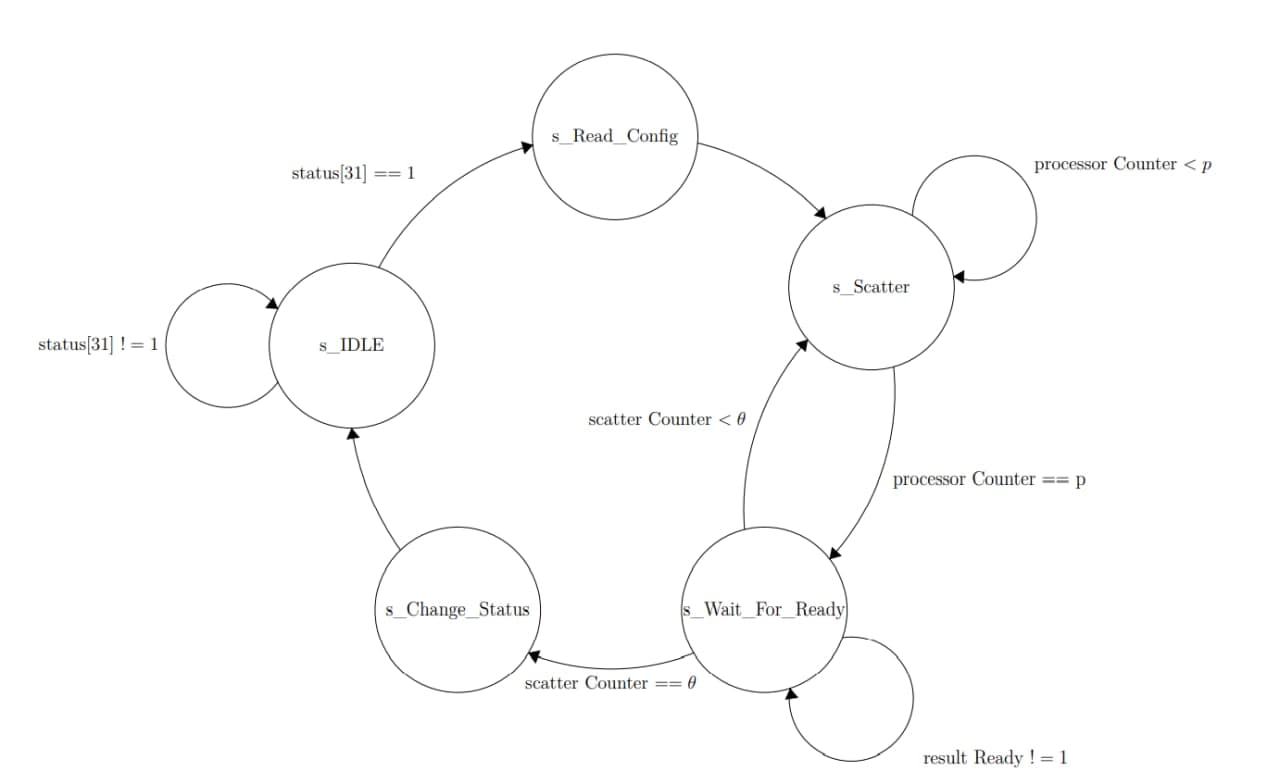
\includegraphics[width=0.92\linewidth]{source/main_cu_fsm.jpg}
	\caption{\lr{Main CU Fsm}}
\end{figure}

\pagebreak

با یک شدن بیت آخر خانه‌ی status در حافظه، این واحد کار خود را آغاز کرده و به پردازنده مرکزی acknowledge می‌دهد که کار خود را آغاز کرده است. 

در حالت بعدی به سراغ خواندن اطلاعات ماتریس‌های ضرب شونده از خانه config در حافظه رفته و این اطلاعات را در رجیستر‌های میانی خود ذخیره می‌کند. پس از آن شروع به پخش کردن بلوک‌های ماتریس‌ها میان پردازنده‌ها کرده که این کار نیز به این صورت انجام می‌شود که منتظر سیگنال acknowledge از طرف پردازنده مورد نظر می‌ماند و اگر این سیگنال را دریافت کند به سراغ پردازنده بعدی می‌رود. این کار را تا زمانی ادامه می‌دهد که به تمامی پردازنده‌ها یک بلوک اختصاص یابد. 

پس از اختصاص بلوک‌ها به تمامی پردازنده ها به حالت بعدی رفته و منتظر می‌ماند تا پردازنده‌ها کار خود را تمام کنند. با تمام شدن کار تمامی پردازنده‌ها، سیگنال result\_ready یک شده و در این حالت اگر بلوکی برای اختصاص دادن باقی‌مانده بود، دوباره به حالت s\_Scatter برگشته و تخصیص را انجام می‌دهد و در غیر اینصورت به حالت بعدی، یعنی s\_Change\_Status رفته و مطابق قرارداد، بیت اول خانه‌ی status حافظه را یک می‌کند که نشان می‌دهد کار ضرب‌ماتریس‌ها تمام شده و نتیجه نیز در حافظه نوشته شده است و پردازنده‌ی مرکزی می‌تواند خروجی را استخراج کند.

\pagebreak

\item 
\lr{Processor}

	\begin{figure}[h]
		\centering
		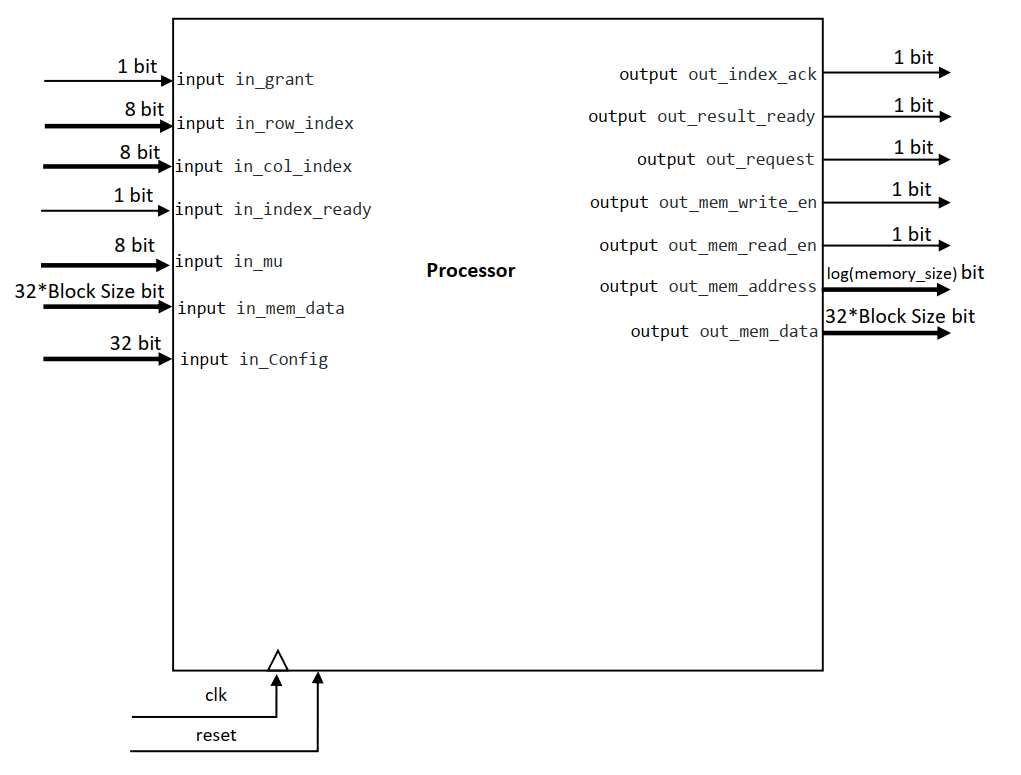
\includegraphics[width=0.55\linewidth]{source/processor.png}
		\caption{\lr{Processor Fsm}}
	\end{figure}

این واحد وظیفه‌ دارد که با دریافت یک $i,j$ و سیگنال‌های ورودی دیگر مقدار $C_{ij}$ را محاسبه کرده و در حافظه ذخیره کند.

در واقع این واحد که متشکل از \lr{Register File} ،
\lr{Control Unit},
\lr{Square Matrix Multiplier}
می‌باشد وظیفه‌ی برقراری اتصالات بین این ماژول‌ها را دارد تا کارهای زیر به درستی انجام شود:

\begin{enumerate}[(I)]
	\item 
	با توجه به \autoref{1}
	آدرس
	  $A_{ix}$ و $B_{xj}$
	  از 	  \lr{Control Unit}  بگیرد و به مموری بدهد سپس متناسب با این اندیس‌ها آدرسی برای \lr{Register File} ایجاد کرده و سیگنال \lr{Write Enable} آن را فعال کند تا \lr{Register File} به درستی این ماتریس‌ها را از حافظه بخواند.
	  
	  \item 
	  بعد از اینکه \lr{Register File} 	  $A_{ix}$ و $B_{xj}$ شد باید سیگنال \lr{Start} را از \lr{Control Unit} گرفته و به \lr{Square Matrix Multiplier} بدهد.
	  
	  \item 
	  داده‌های مورد نیاز \lr{Square Matrix Multiplier} را در کلاک‌های مختلف از \lr{Register File} خوانده تا عملیات ضرب ماتریس مربعی 	  $A_{ix}\times B_{xj}$ به درستی انجام شود.
	  
	  \item 
	  بعد از اتمام ضرب حاصل را با مقادیر قبلی که در رجیستر فایل برای $C_{ij}$ بود جمع بزند.
	  
	  \item
	 بعد از اینکه عملیات‌های بالا به اندازه‌ی $\mu$ بار تکرار شد سیگنال مناسبی برای \lr{Main Control Unit} ارسال کند تا در صورت نیاز \lr{Main Control Unit} محاسبه‌ی بلوک دیگری را به این پراسسور اختصاص دهد.
	   
	
\end{enumerate}
	
\pagebreak

	\item 
	\lr{Control Unit}

\begin{figure}[h]
	\centering
	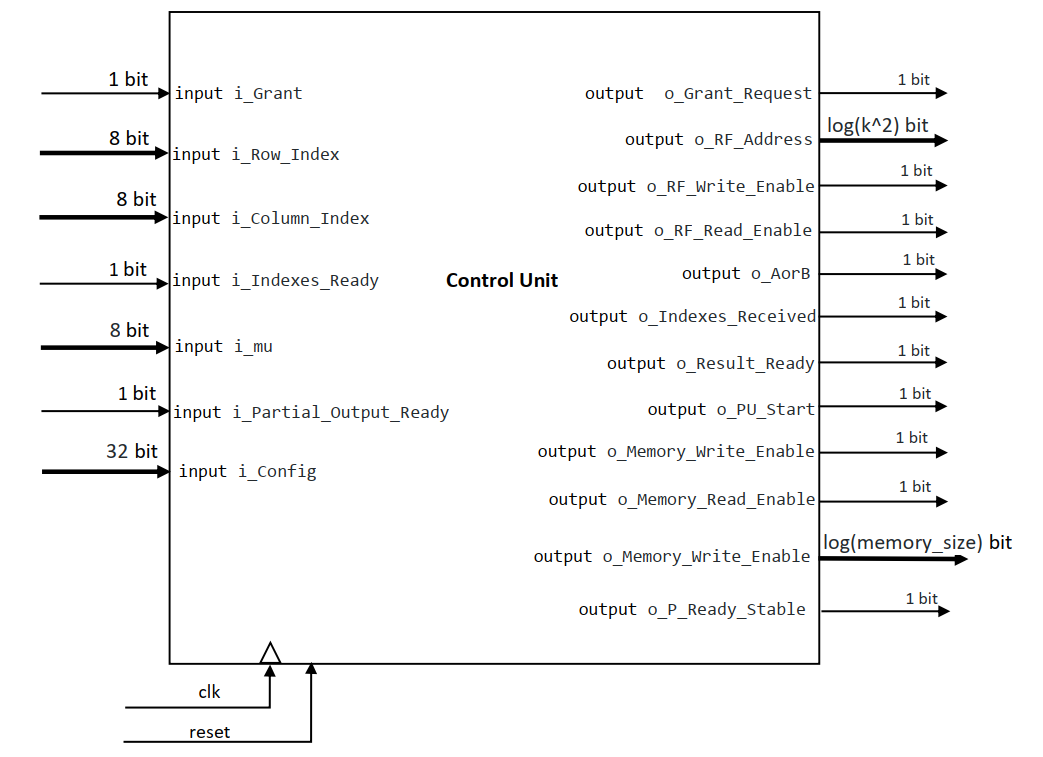
\includegraphics[width=0.6\linewidth]{source/control_unit.png}
	\caption{\lr{CU Fsm}}
\end{figure}
	
	این ماژول وظیفه‌ی کنترل سیگنال‌ها هنگام محاسبه‌ی \autoref{1} را دارد.
	در واقع این ماژول با پیاده کردن دیاگرام حالت زیر مقدار $x$ را تغییر می‌دهد و هر بار $A_{ix},B_{xj}$ جدید را از حافظه‌ می‌خواند و سپس آن را به واحد ضرب کننده‌ی ماتریسی می‌دهد و پس از اینکه جواب نهایی حاضر شد آن را در حافظه می‌نویسد.
	\begin{figure}[h]
		\centering
		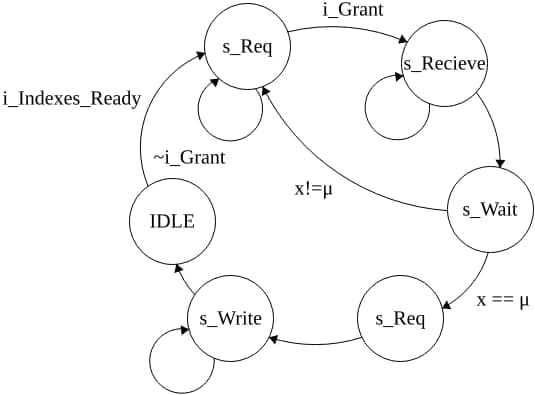
\includegraphics[width=0.53\linewidth]{source/fsm_cu.jpg}
		\caption{\lr{CU Fsm}}
	\end{figure}
\\
همانطور که مشخص است این واحد بعد از دریافت اندیس‌های اصلی $i,j$ از \lr{Arbiter} اجازه‌ی نوشتن در \lr{Address Bus} را می‌خواهد و بعد از دریافت کردن آن به اندازه‌ای در حالت \lr{Receive} می‌ماند تا $A_{ix}$ و $B_{xj}$ به طور کامل در رجیستر فایل نوشته شوند و این کار را به انداز‌ه‌ی $\mu$ بار تکرار می‌کند تا نهایتا $C_{ij}$ محاسبه شود.
	
	\item 
	\lr{Matrix Multiplier}
	
	\begin{figure}[h]
		\centering
		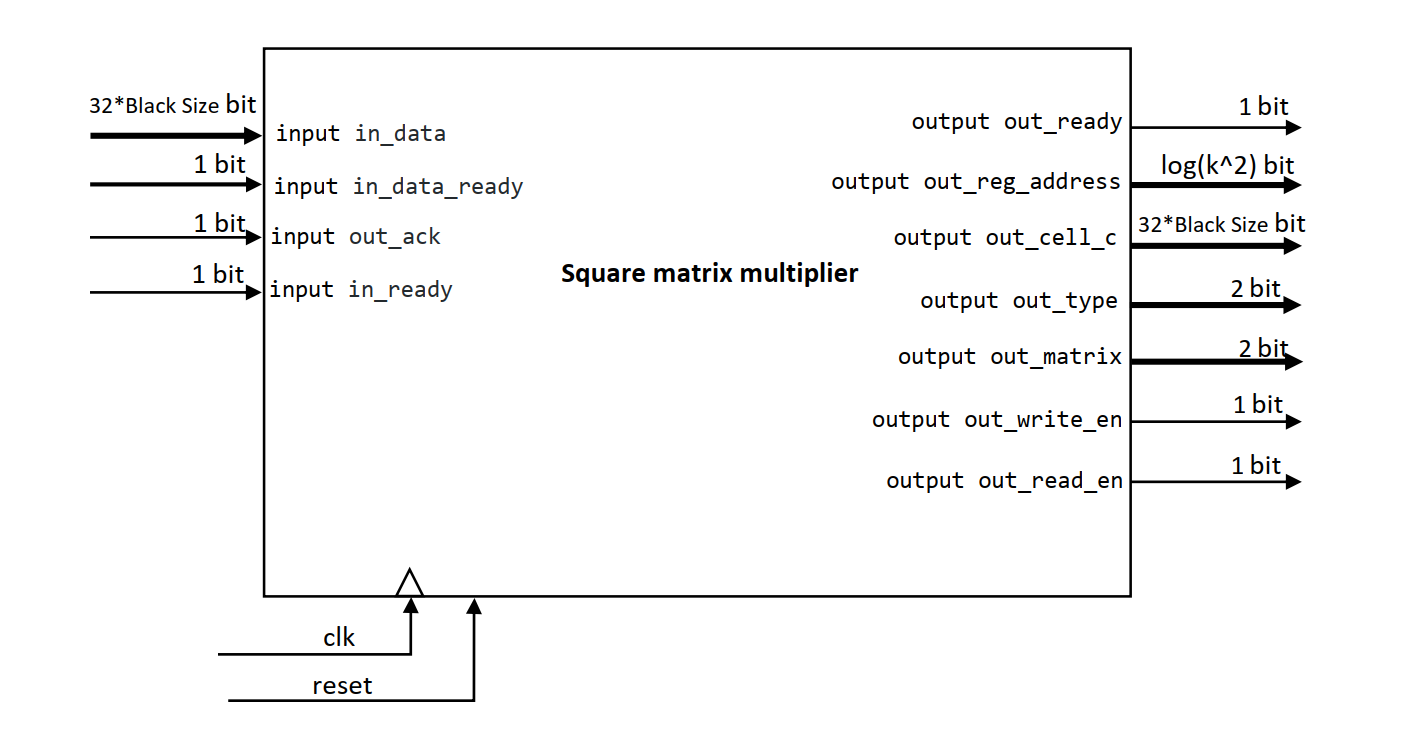
\includegraphics[width=0.7\linewidth]{source/squareMatrixMult.png}
		\caption{\lr{Square Matrix Multiplier Schematic}}
	\end{figure}

	
	این واحد دو ماتریس $k*k$ را با توجه به نمودار حالت زیر ابتدا از رجیستر فایل می‌خواند و سپس در هم ضرب می‌کند:
	\begin{figure}[h]
		\centering
		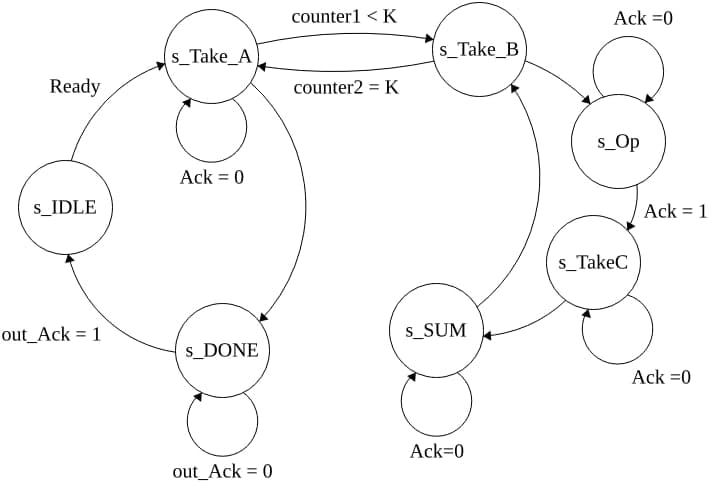
\includegraphics[width=0.6\linewidth]{source/fsm_sq_mat.jpg}
		\caption{\lr{Square Matrix Multiplier Fsm}}
	\end{figure}
	\\ در حالت اول با دریافت بیت \lr{in\_Ready} که از طرف واحد کنترلی فرعی می‌آید مشخص می‌شود که باید مراحل ضرب کردن را آغاز کند. با آمدن این بیت در دو حالت \lr{Take A} و\lr{Take B} می‌ماند تا یک سطر و یک ستون را در یافت کند سپس در مرحله‌ی \lr{Operation} این سطر و ستون را به واحد‌های کوچک‌تری که مربوط به ضرب سطر و ستون می‌باشند میدهد و این کار را تا زمانی که تمام درایه‌ها را محاسبه کند ادامه می‌دهد. و نهایتا خروجی را در مرحله‌ی \lr{Done} درون رجستر فایل می‌ریزد.


\pagebreak


\item 
\lr{Index To Address Transformer}

	\begin{figure}[h]
	\centering
	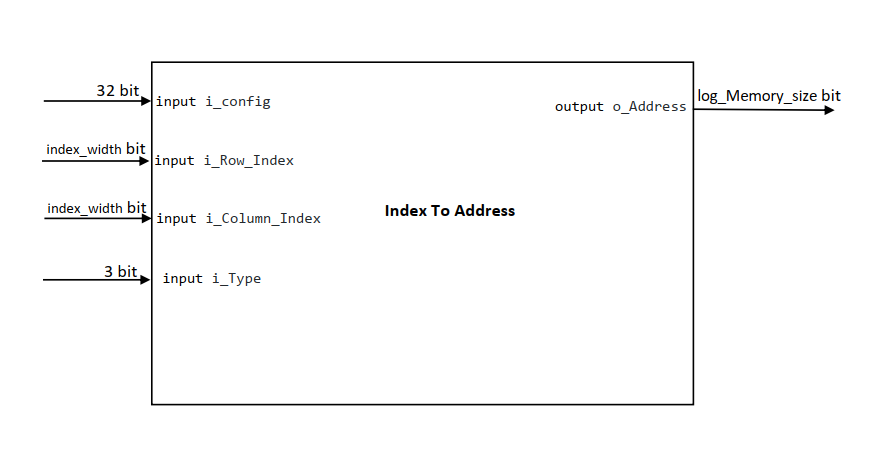
\includegraphics[width=0.8\linewidth]{source/index_to_address.png}
	\caption{\lr{Index To Address Transformer Schematic}}
	\end{figure}


	این واحد با داشتن کانفیگ و همچنین ورودی‌های مشخص کننده‌ی دیگر باید بتوانند آدرس $A_{ix}$ یا $B_{xj}$ و یا $C_{ij}$ را پیدا کند بیت‌های ورودی این واحد شامل اندیس سطر و ستون و ۳ بیت دیگر که مشخص می‌کند باید آدرس کدام یک از $A,B,C$ را پیدا کند. 
	
	روشن است که عملکرد این واحد به قرار داد اولیه‌ای که برای حافظه و کانفیگ گذاشتیم به شدت وابسته خواهد شد و می‌توان آن را تنها با توجه به حالت‌های مختلف برای \lr{i\_Type} محاسبه کرد.
	
	\pagebreak
	
	\item \lr{Column Processor}
	
\begin{figure}[h]
	\centering
	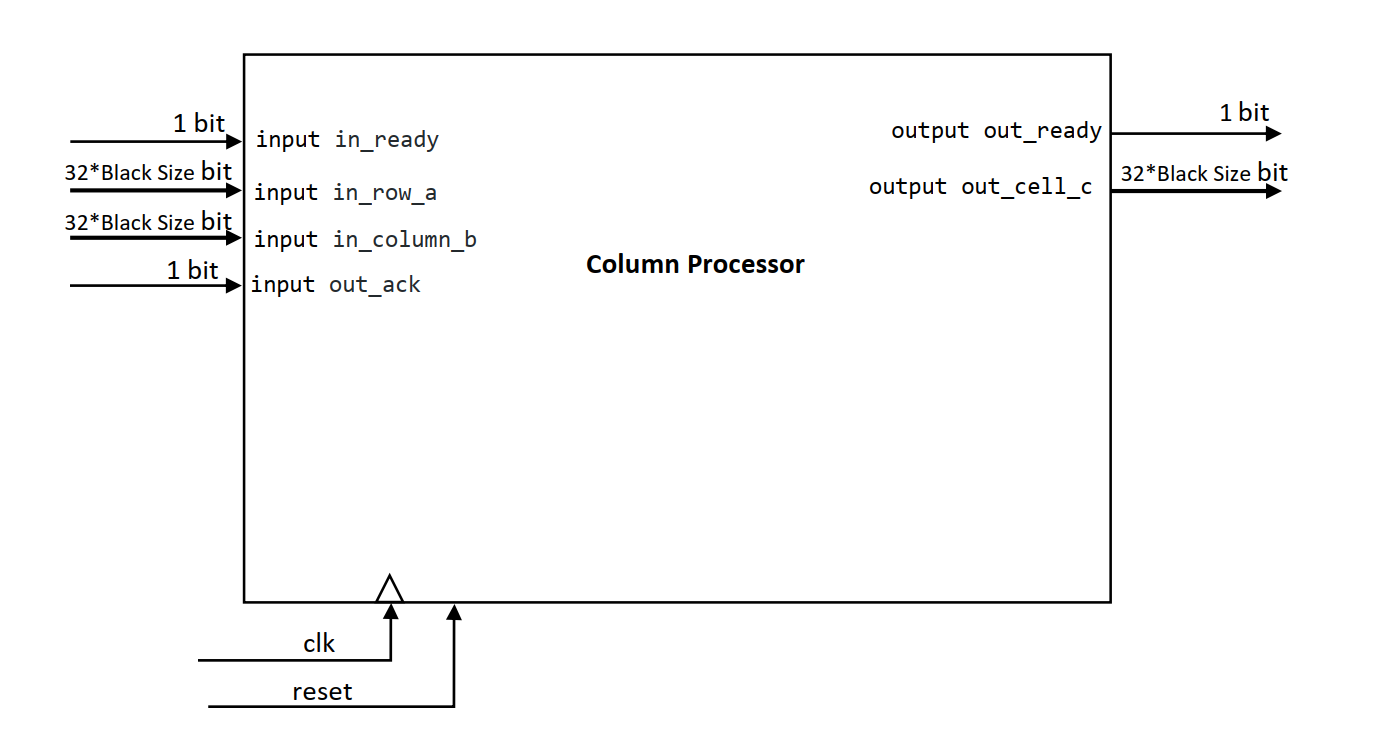
\includegraphics[width=0.7\linewidth]{source/columnProcessor.png}
	\caption{\lr{Column Processor Schematic}}
\end{figure}
	
	این واحد به منظور محاسبه‌ی ضرب یک سطر از ماتریس $A_{ix}$ در یک ستون از ماتریس $B_{xj}$ طراحی شده است. 


	\begin{figure}[h]
		\centering
		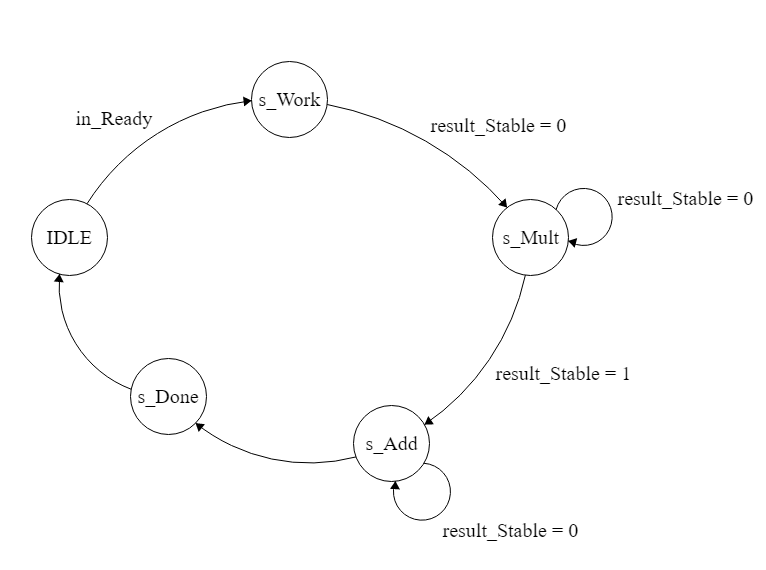
\includegraphics[width=0.6\linewidth]{source/column_procsessor.png}
		\caption{\lr{Column Processor Fsm}}
	\end{figure}

هر موقع واحد \lr{Square Matrix Multiplier} داده‌های این واحد را فراهم کند بیت \lr{in\_Ready} را برایش فعال می‌کند سپس این واحد نیز داده‌ها را ابتدا در اختیار واحد ضرب کننده‌ی سطری می‌دهد و بعد از آماده شدن پاسخ آن داده‌ها را در اختیار واحد جمع کننده قرار می‌دهد و در نهایت این داده‌ها را در محل مناسبی در \lr{Register File} می‌ریزد.

\pagebreak

\item \lr{Column Multiplier}

	\begin{figure}[h]
	\centering
	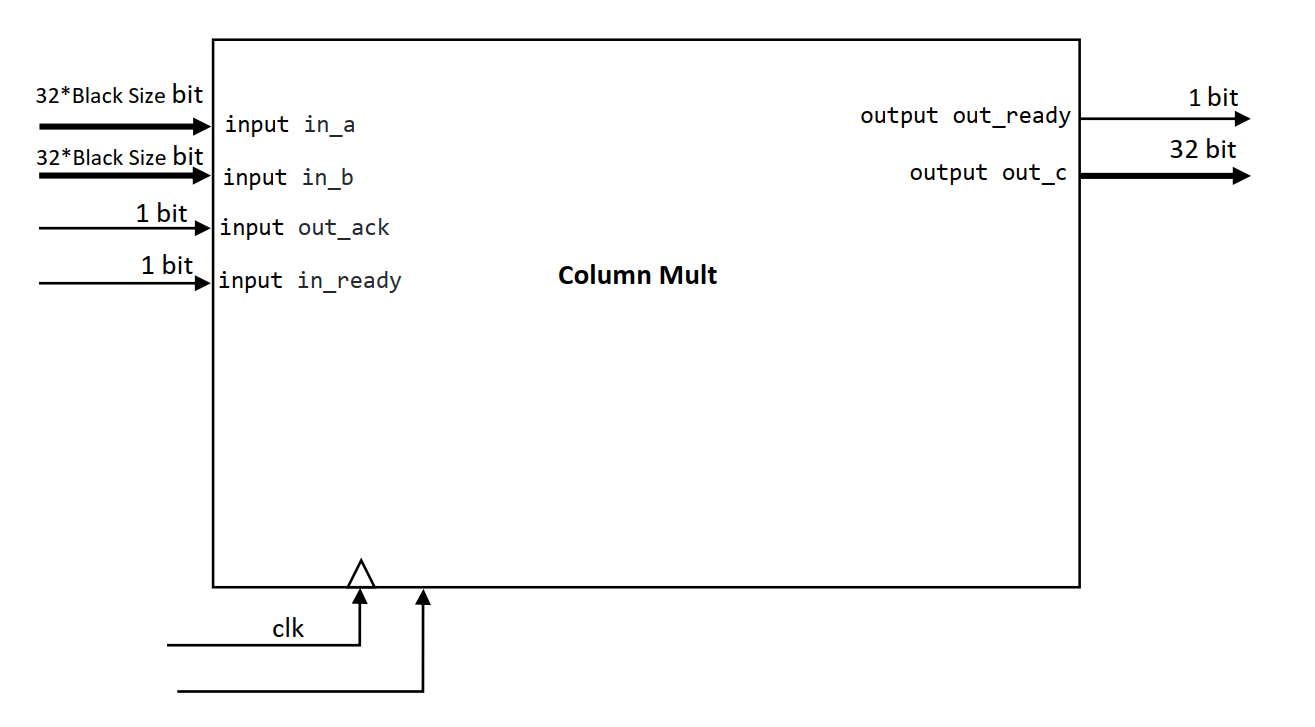
\includegraphics[trim={0 2cm 0 0}, clip, width=0.7 \linewidth]{source/columnMult.png}
	\caption{\lr{Column Multiplier Schematic}}
	
\end{figure}

وظیفه‌ی این واحد جمع کرد این است که حاصل ضرب نقطه‌ای یک سطر از $A_{ix}$ و یک ستون از $B_{xj}$ را محاسبه کرده و این مقدار را نگه داشته تا \lr{column\_processors} بتواند از آن استفاده کند. 

	\begin{figure}[h]
	\centering
	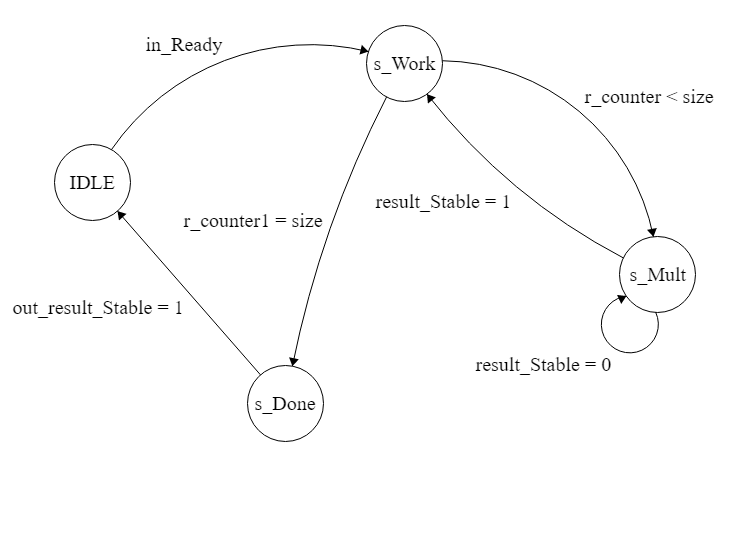
\includegraphics[trim={0 2cm 0 0}, clip, width=0.7 \linewidth]{source/column_mult.png}
	\caption{\lr{Column Multiplier Fsm}}

\end{figure}

همانطور که از نمودار حالت مشخص است این واحد تا زمانی که \lr{r\_Counter} از $k$ کوچک‌تر باشد ضرب کردن را تکرار می‌کند و بعد از آن به حالت \lr{s\_Done} می‌رود.
	
\pagebreak

\item \lr{Column Adder}

	\begin{figure}[h]
	\centering
	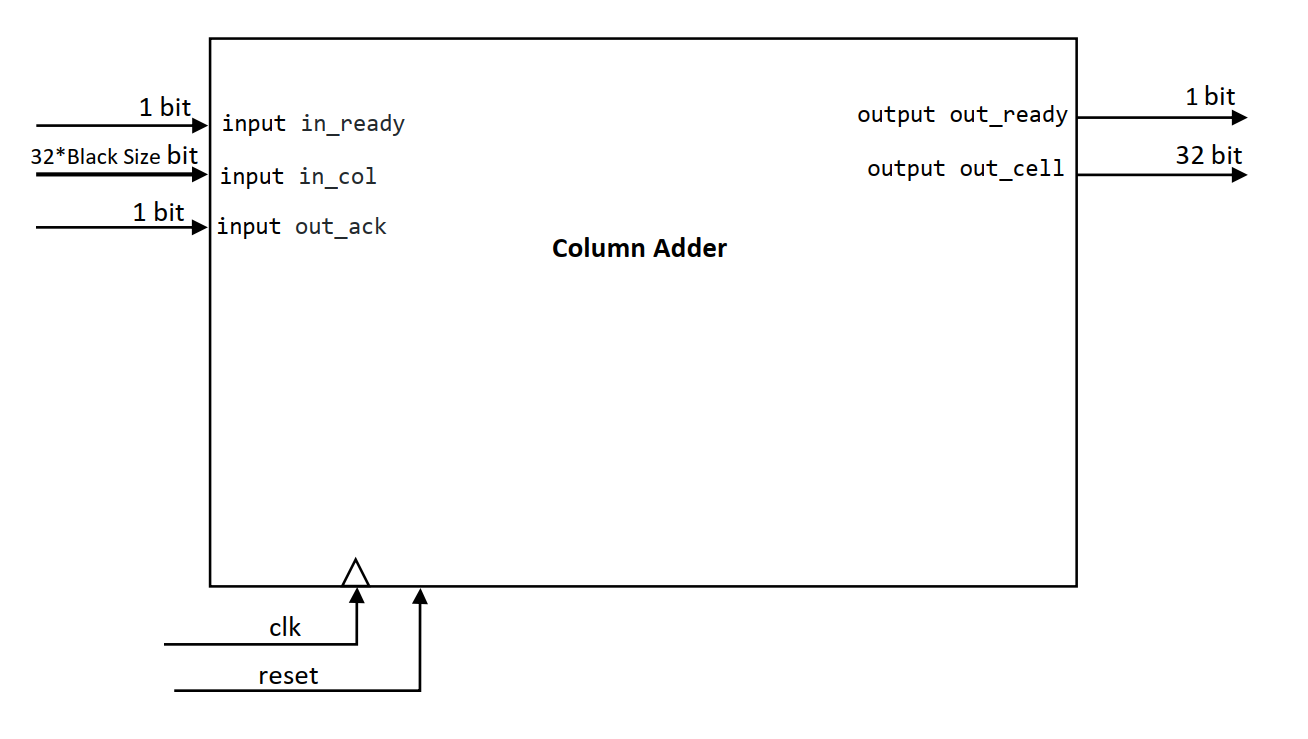
\includegraphics[trim={0 2cm 0 0}, clip, width=0.7 \linewidth]{source/columnAdder.png}
	\caption{\lr{Column Adder Schematic}}
	
\end{figure}

این واحد وظیفه‌ی جمع کردن یک ستون در ورودی را دارد.

	\begin{figure}[h]
	\centering
	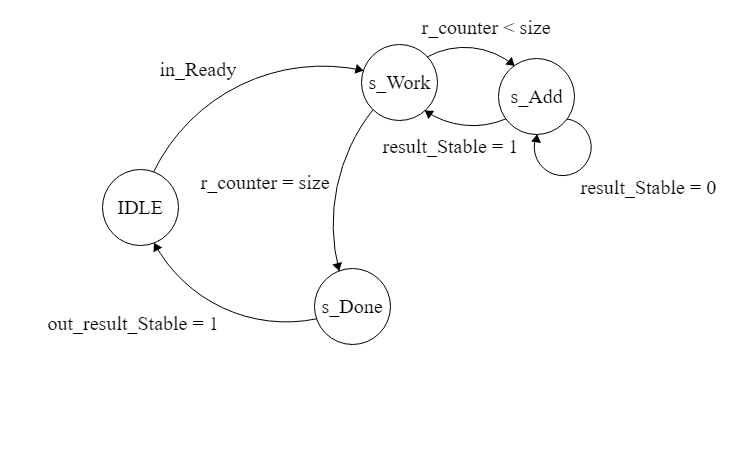
\includegraphics[trim={0 2cm 0 0}, clip, width=0.7 \linewidth]{source/column_adder.png}
	\caption{\lr{Column Adder Fsm}}
	
\end{figure}

همانطور که می‌توان از این نمودار حالت دید نحوه‌ی عملکرد این واحد به گونه‌ایست که با دریافت سیگنال \lr{in\_ready} در حالت جمع کردن بلاک‌ها قرار می‌گیرد و این کار را تا زمانی که \lr{r\_counter} از $k$کمتر باشد ادامه می‌دهد.
	
\end{itemize}

\pagebreak

\subsection{شماتیک کلی سخت‌افزار}

در این بخش بعد از سنتز به وسیله‌ی \lr{XilinX}  شماتیک کلی سخت ‌‌افزار را استخراج کردیم که به صورت زیر می‌باشد.

	\begin{figure}[h]
	\centering
	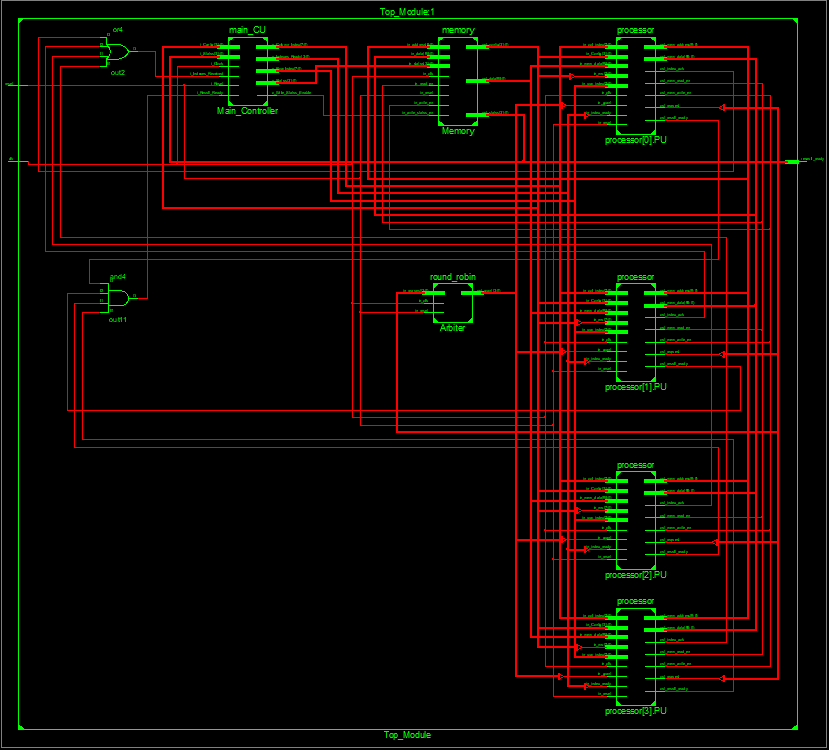
\includegraphics[width=0.95\linewidth]{source/scheeem.png}
	\caption{شماتیک نهایی \lr{Top Module}}
\end{figure}


\pagebreak


\pagebreak
\section{روند شبیه‌سازی و نتایج حاصل}
\subsection{توصیف \lr{TestBench}ها}
\subsection{توصیف روند کلی شبیه‌سازی}
\subsection{توصیف \lr{Golden Model}}
\subsection{مقایسه‌ی خروجی‌های نهایی با \lr{Golden Model}}

\section{پیاده‌سازی و نتایج حاصل}

با استفاده از نرم افزار ISE سنتز انجام گرفت که نتایج آن در ادامه گزارش آمده است.
به کمک سنتز موفق تعداد ثبات های استفاده شده، تعداد LUTها و حداقل تعداد کلاک به طوری که سیستم دچار مشکلات زمان بندی نشود را به دست می آید.

\end{document}







